{
\nofooter \noheader \frame[noframenumbering]{\titlepage}
}
{
\frame{\frametitle{Outline}\label{TableOfContents}
\setcounter{tocdepth}{2}\tableofcontents}
}

\section{Library Overview}
\begin{frame}{Vision (the ambitious version)}
  \begin{itemize}
  \item Provide an \textbf{easy to use}, \textbf{customizable} and
    \textbf{extendable} open source library for UQ problems, both
    forward and inverse.
  \item Multilevel and Multi-index versions of Monte Carlo, Quasi Monte
    Carlo, Stochastic collocation, Least square projection among
    others.
  \item Support parallel computation whenever possible.
  \item Provide easy to use storage facility.
  \item Provide easy to customize plotting facility (for common
    plots).
  \item Provide easy to run test cases.
  \item Use \texttt{Python} for easier implementation of most parts of code
    and use object code (\texttt{C++} or \texttt{FORTRAN}) for
    computationally expensive parts.
  \end{itemize}
\end{frame}

\begin{frame}{What has been done, \lib~\texttt{0.2.0.dev0}}
  \begin{itemize}
  \item Multilevel and Multi-index versions of Monte Carlo.
  \item Provide easy to use storage facility in MySQL.
  \item Provide easy to customize plotting facility (for common
    plots).
  \item Provide easy to run test cases.
  \item Documentation is still in progress (these slides are part of it).
  \item Interface is written with the other features in mind.
  \end{itemize}
\end{frame}

\begin{frame}
\centering
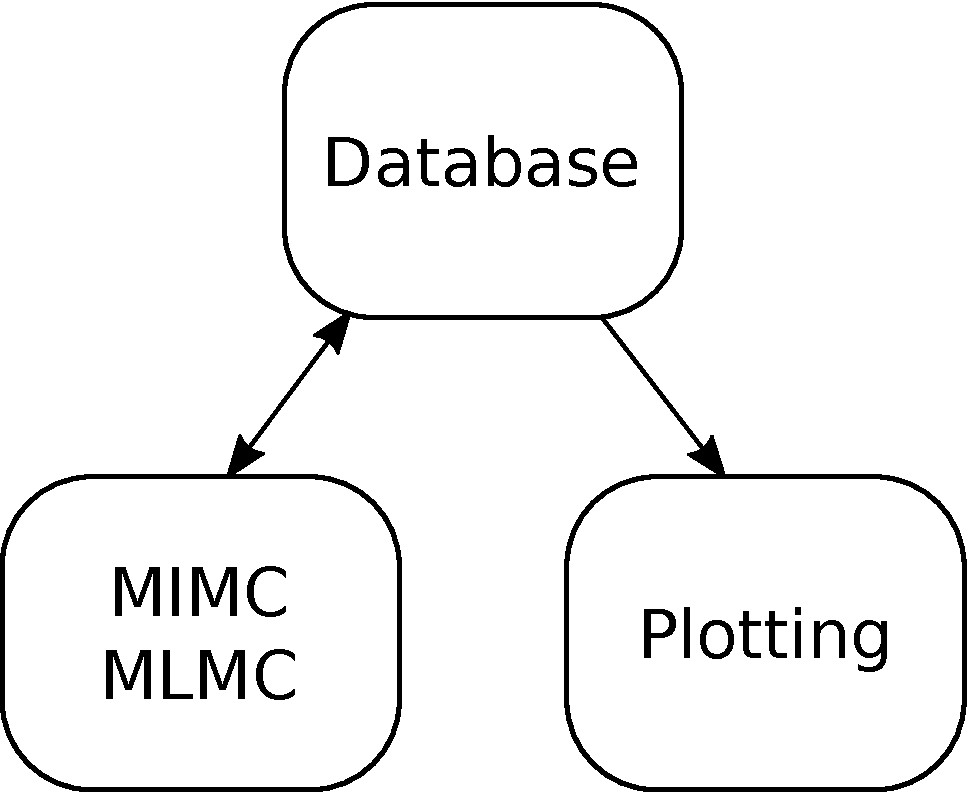
\includegraphics[scale=0.4]{src/imgs/scheme}
\end{frame}

\begin{frame}{Why?}
  \begin{itemize}
  \item \texttt{Python}
    \begin{itemize}
    \item Open source. No need for licensing
    \item An easy to use programming language. Familiar to
      \texttt{MATLAB} users (Especially with \texttt{numpy} and \texttt{matplotlib})
    \item Can call object code for computationally expensive parts,
      e.g., samplers.
    \end{itemize}
    \item \texttt{MySQL}
      \begin{itemize}
      \item Relatively easy data modifications and querying.
      \item Allows asynchronous access which is ideal for parallel computation.
      \item Allows remote access.
      \item Optimal storage and data querying.
      \end{itemize}
    \end{itemize}
\end{frame}

\section{Primer}
\subsection{Problem}
\begin{frame}\frametitle{The central question}
  Given an $\rset^n$-valued random variable, $\vec X$ with PDF
  $f(\vec x) : \rset^n \to [0,\infty)$ and a function,
  $\func : \rset^n \to \rset$, assume that we are interested in
  computing the quantity
\begin{equation*}\label{eq:expectation}
  \E{\func(\vec X)} = \int_{\rset^n} \func(\vec x) f(\vec x) \di{\vec x}.
\end{equation*}
\pause
\vskip 0.5cm \textbf{Possible difficulties:}
\begin{itemize}
\item PDF, $f$, is inaccessible, only (approximate) samples of $\vec X$ can be generated.
\begin{itemize}
\item E.g., $\vec X$ is the solution of an SDE.
\end{itemize}
% \item $\func$ cannot be computed exactly or cheaply.
%   % RAUL: $\func$ is the easy part, it is X the difficult one.  I suggest
%   % you emphasize in the second point that the expectation must be
%   % approximated
% \begin{itemize}
% \item E.g., Finite Element Method approximation to a PDE solution.
% \end{itemize}
\item Dimension, $n$, is large or even infinite, hence the integral is expensive to approximate.
\begin{itemize}
\item E.g., expansion of a random field.
\end{itemize}
\end{itemize}
\end{frame}

\begin{frame}{Setup} % SOME FRAME
  Our objective is to build an estimator $\mathcal{A} \approx
  \E{\func (\vec X)}$ with
  \red{minimal work} where
  \begin{equation*}
    % \prob{
    P(
    |\mathcal{A} - \E{\func(\vec X)}| \leq \red{ \tol}
    )\
    % }\
    \ge \epsilon
  \end{equation*}
  %
  for a given accuracy $\tol$ and a given confidence level determined
  by $0 < \epsilon < 1$. \pause

  Instead, we impose the following, more restrictive, two constraints:
  \begin{align*}
    \text{\bf Bias constraint:} & &|\E{\mathcal{A}-\func (\vec X)}| \leq (1-\theta)
                                    \tol, \\
%\begin{overlayarea}{\textwidth}{5in}
\text{\bf Statistical constraint:}& &
\Alt<2>{P\left( |\mathcal{A} - \E{\mathcal{A}}| \leq \theta\tol \right) \ge \epsilon.}
{\var{\mathcal{A}} \leq \op*{\frac{\theta
      \tol}{\Phi^{-1}\op*{\frac{\epsilon + 1}{2}}}}^2.}
%\end{overlayarea}
  \end{align*}
  For some tolerance splitting, $\theta \in (0,1)$. \uncover<3>{Assuming (at least
    asymptotic) normality of the estimator, $\mathcal{A}$. Here,
    $\Phi^{-1}$ is the inverse of the standard normal CDF.}
\end{frame}


\begin{frame}<1>[label=MCNotation]\frametitle{Numerical approximation}
  {\bf Notation:} $\func_{\Alt<2>{\valpha}{\ell}}$ for
  $\Alt<2>[c]{\valpha \in \nset^d}{\ell \in \nset}$ is the
  approximation of $\func$ calculated based on
  discretization parameters
  ${\vec h_{\Alt<2>{\valpha}{\ell}}} =
\left( h_{\Alt<2>[c]{\alpha_i}{\ell, i}} \right)_{i=1}^d$.
\begin{center}
  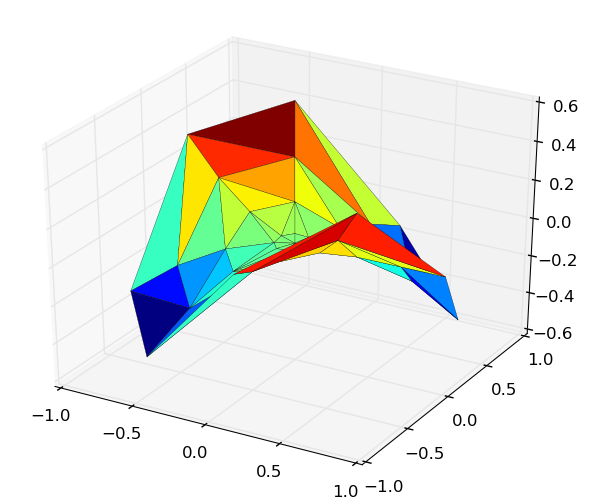
\includegraphics[scale=.2]{mlmc_1}
  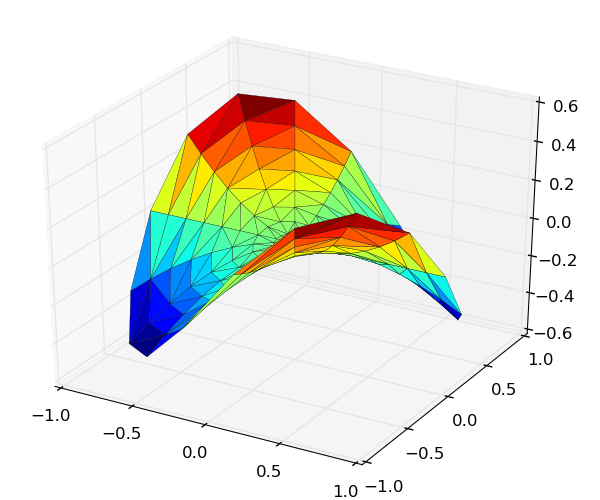
\includegraphics[scale=.2]{mlmc_2}
  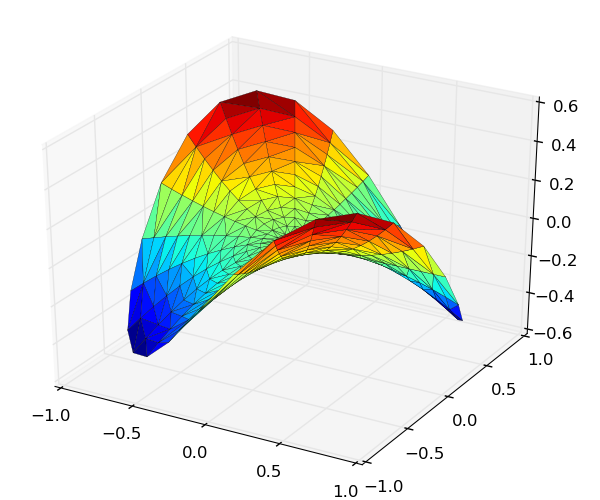
\includegraphics[scale=.2]{mlmc_3}
\end{center}

\end{frame}

\subsection{Monte Carlo (MC)}
\begin{frame}[label=MC]\frametitle{Monte Carlo}
The simplest (and most popular) estimator is the Monte Carlo estimator
\[\estmc{\func_L ; M} =  \frac{1}{M}\sum_{m=1}^M {\func}_{L}(\vec
  X^{\op{m}}), \] for a given level, $L$, and number of
samples, $M$, that we can choose to satisfy the error constraints and
minimize the work.
% \[ \var{\estmc{\func_L ; M}} = \frac{\var{g_{L}}}{M} \pause
% \leq \left( \frac{\theta \tol}{{\Phi^{-1}\op*{\frac{\epsilon + 1}{2}}}} \right)^2 \]
% To satisfy the variance constraint, we have to choose $M = \Order{\tol^{-2}}$.
\end{frame}
% %%%%%


\begin{frame}{MLMC main idea: Variance reduction}
\centering
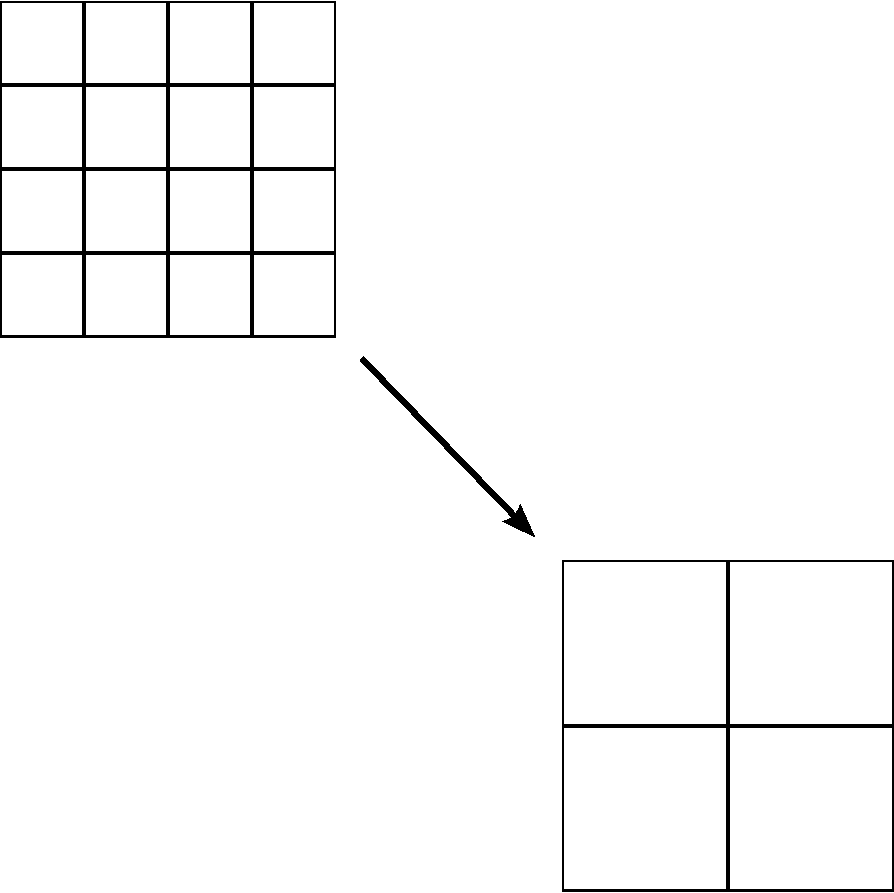
\includegraphics[scale=0.4]{src/imgs/mesh_mlmc}
\end{frame}


\begin{frame}<0>[label=MCAssumptions]\frametitle{Assumptions}
  \only<1->{
    {\bf Assumption MC${\mathbf 1}$ (Bias):}
    $\displaystyle\hfill \left|\E{\func - \func_{\ell}}\right|
    \lesssim \exp\op{-w\ell},$

  {\bf Assumption MC${\mathbf{2}}$ (Work):}
  $\displaystyle
   \hfill \work{\func_{\ell}} \lesssim \exp\op{\alt<5->{\red{d}}{d} \gamma \ell},$

     \uncover<3->{
    {\bf Assumption MLMC${\mathbf 3}$ (Variance):}
$\displaystyle
    \hfill  \var{\func_{\ell} - \func_{{\ell-1}}} \lesssim \exp\op{-s \ell}
$}
\vskip 0.2cm
for all $\ell \in \nset$ and positive constants $\gamma,
w\only<3->{, s}$.}


{
\vskip 0.5cm
\uncover<5>{\textbf{Recall}:}
\uncover<1-2, 5>{
Optimal cost of Monte Carlo is $\Order{\tol^{-2 -\frac{\alt<5->{\red{d}}{d} \gamma}{w}}}$}
\vskip 0.5cm
\uncover<4->{
The optimal work of MLMC is
\begin{equation*}
\begin{cases}
\Order{\tol^{-2}} & s > \alt<5->{\red{d}}{d} \gamma\\
\Order{\tol^{-2}} \left(\log\op*{\tol^{-1}}\right)^2& s = \alt<5->{\red{d}}{d} \gamma\\
\Order{\tol^{-2-\frac{\alt<5->{\red{d}}{d}\gamma-s}{w}}} & s < \alt<5->{\red{d}}{d} \gamma
\end{cases}
\end{equation*}
}

\uncover<5->{\textbf{Notice:} the cost exponentially increases with increasing $\alt<5->{\red{d}}{d}$.}
}
\end{frame}

\subsection{Multilevel Monte Carlo (MLMC)}
\begin{frame}{Multilevel Monte Carlo (MLMC){\quad \tiny (Heinrich, 1998) and (Giles, 2008)}}
  Observe the telescopic identity
  \[
    \E{\func} \approx \E{\func_{L}} = \E{\func_{0}} +
    \sum_{{\ell}=1}^{L} \E{\func_{\ell} -
      \func_{{\ell - 1}}} \pause
= \sum_{{\ell}=0}^{{L}} \E{ \Delta_\ell \func}, \]
where
  \begin{align*}
    \Delta_\ell \func = \begin{cases}
      \func_{0} & \text{if } \ell=0, \\
      \func_{{\ell}} -   \func_{{\ell-1}} & \text{if } \ell> 0.
      \end{cases}
    \end{align*}
    \pause Then, using Monte Carlo to approximate each difference independently, the
    MLMC estimator can be written as
    \begin{align*}
      \estmlmc{\func ; L} = \sum_{{\ell}=0}^{{L}} \estmc{\Delta
      \func_\ell ; M_\ell}.
    \end{align*}
    Main idea: variance reduction using cheaper approximations.
\end{frame}

\begin{frame}\frametitle{Optimal number of samples}
Given the following estimates
\begin{equation*}
  V_\ell = \begin{cases} \var{\func_{0}} & \ell = 0, \\
\var{\func_{{\ell}} - \func_{{\ell-1}}} & \ell \geq 1, \\
\end{cases}
\end{equation*}
\begin{equation*}
  W_\ell = \begin{cases} \text{Work of a single sample of } {\func_{0}} & \ell = 0, \\
\text{Work of a single sample of } (\func_{{\ell}} - \func_{{\ell-1}}) & \ell \geq 1. \\
\end{cases}
\end{equation*}
Then, using simple Lagrangian optimization of the total work subject to
the variance constraint then, we can obtain the optimal number of samples
\[ M_\ell \approx \op*{\frac{\theta
      \tol}{\Phi^{-1}\op*{\frac{\epsilon + 1}{2}}}}^{-2}{
    \sqrt{\frac{V_\ell}{W_\ell}}\left(\sum_{i=0}^L \sqrt{V_i
        W_i}\right) },\quad \text{for }0\le \ell \le L. \]
\end{frame}


\againframe<3->{MCAssumptions}

\begin{frame}\frametitle{Continuation MLMC}
\begin{itemize}
\item To compute $M_\ell$ we need to find $L$ and find estimates of
  $V_\ell$.
\pause
    \item Instead of running for the small required $\tol$, CMLMC runs
      a sequence of MLMC realizations, for decreasing
      tolerances, ending with the required $\tol$.
    \item In each step, estimates of $V_\ell$ are generated using a
      Bayesian setting which uses {\bf Assumption MLMC3} coupled with
      the generated samples to produce good estimates even with a
      small number of samples.
    \item The value of $L$ is also chosen in each step to minimize the
      work. This allows choosing a better splitting parameter,
      $\theta$.
    \item CMLMC does not have to reuse samples between iterations,
      ensuring an unbiased estimator for level $L$ approximation.
  \end{itemize}
\end{frame}


\section{Installation}

\begin{frame}{\lib~showcase}
  \begin{itemize}
  \item Code required for basic MLMC run.
  \item Show single run of \lib.
  \item Show plots in pdf.
  \item Show database in mysql.
  \end{itemize}
\end{frame}

\begin{frame}[fragile]{Installation}
\begin{itemize}
  \item Prerequisites: \texttt{gcc} (supporting \texttt{c++11}), \texttt{python2.7}, \texttt{pip}, \texttt{mysql-server}, \texttt{mysql-client}.
  \item First step:
\begin{verbatim}
> git clone \
      https://github.com/StochasticNumerics/mimclib.git
> cd mimclib
> make pip
\end{verbatim}
  \item Note: to update to latest version
\begin{verbatim}
> git pull
\end{verbatim}
\item Done! Sort of.
\end{itemize}
\end{frame}

\begin{frame}[fragile]{Setting up the database}
  \begin{itemize}
  \item Make sure \texttt{mysql-server}, \texttt{mysql-client}, and
    \texttt{libmysqlclient-dev} are installed on your data server.
  \item Create \texttt{mimclib} database on data server
\begin{verbatim}
> python -c 'from mimclib.db import MIMCDatabase ; \
         print MIMCDatabase().DBCreationScript();' \
         | mysql -u root -p
\end{verbatim}
\item Create database user for \lib~(hint: you can use local username)
\begin{verbatim}
     > mysql -u root -p
mysql> CREATE USER 'USER'@'%' \
              IDENTIFIED BY 'password';
mysql> GRANT ALL PRIVILEGES ON mimc.* TO \
             'USER'@'%' WITH GRANT OPTION;
\end{verbatim}
  \end{itemize}
\end{frame}

\begin{frame}[fragile]{Other useful \texttt{MySQL} commands}
  \begin{itemize}
  \item Change password
\begin{verbatim}
     > mysql -u USER -p
mysql> SET PASSWORD FOR 'USER'@'%' \
       = PASSWORD('newpassword');
\end{verbatim}
  \end{itemize}
\end{frame}

\begin{frame}{MIMC Database}
\centering
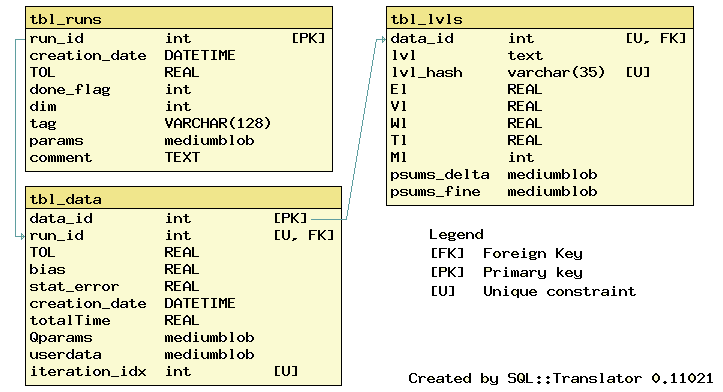
\includegraphics[scale=0.6]{src/imgs/db_schema}
\end{frame}

\begin{frame}[fragile]{Installation for Debian/Ubuntu}
\begin{itemize}
  \item
\begin{verbatim}
> git clone \
      https://github.com/StochasticNumerics/mimclib.git
> cd mimclib
> ./mimc_install.sh
\end{verbatim}
  \item Updates all packages on the system
  \item Installs all prerequisites
  \item Clones and installs the library
  \item Creates a database with the current user and no password.
  \item Standard GBM Example is ready to run.
\end{itemize}
\end{frame}


\section{GBM Example}
\begin{frame}{Problem setup: Geometric Brownian Motion}
Given $S(0), \mu$ and $\sigma$, define
  \[
    S(t) = S(0) + \mu \int_{0}^T S(t) \di{t} + \sigma \int_{0}^T S(t) \di{W}(t)
\]

We can find (using It\^o integral and a log transformation)
\[\aligned
\E{S(t)} &= S(0) e^{\mu t}\\
\var{S(t)} &= \op*{S(0)}^2 e^{2 \mu t} \op*{e^{\sigma^2 t} - 1}
\endaligned\]
\end{frame}

\begin{frame}{The end}
  \begin{itemize}
  \item Slides can be found on GitHub under {``docs''}
    \url{https://github.com/StochasticNumerics/mimclib}.
    \item You can post questions in the ``Issues'' page.
  \item Next time
    \begin{itemize}
    \item Next, next time: Multi-index Monte Carlo applied on PDEs in
      3D.
    \end{itemize}
  \end{itemize}
\end{frame}

% \begin{frame}[fragile]{A typical python example for a single MLMC run}
% \begin{verbatim}
% # Read arguments from command line
% import argparse
% parser = argparse.ArgumentParser(add_help=True)
% mimc.MIMCRun.addOptionsToParser(parser)
% tmp = parser.parse_known_args()[0]
% mimcRun = mimc.MIMCRun(**vars(tmp))

% # Create entry in DB for MIMCRun
% db = mimcdb.MIMCDatabase()
% run_id = db.createRun(mimc_run=mimcRun,
%                       tag="MyFirstMIMCRun")
% \end{verbatim}
% \end{frame}

% \begin{frame}[fragile]{User defined functions with typical impl.}
% \begin{verbatim}

% def myItrDone(itrIndex, TOL, totalTime)
%     db.writeRunData(run_id, mimcRun,
%                     itrIndex, TOL, totalTime)

% def mySampleLvl(moments, mods, inds, M):
%     ...

% mimcRun.setFunctions(fnSampleLvl=mySampleLvl,
%                      fnItrDone=myItrDone)

% mimcRun.doRun()
% print("Final value:", mimcRun.data.calcEg())
% \end{verbatim}
% \end{frame}

% \begin{frame}[fragile]{Minimal example of \texttt{fnSampleLvl}}
% \begin{verbatim}
% def mySampleLvl(moments, mods, inds, M):
%     tic = time.time()
%     psums = np.zeros(len(moments))
%     for m in range(0, M):
%         rf = SampleRandomField()
%         solves = np.array([SolvePDE(rf, ind)
%                            for ind in inds])
%         psums += np.sum(mods*solves)**moments
%     return psums, time.time() - tic
% \end{verbatim}
% \end{frame}


% \begin{frame}[fragile]{Running the script. MLMC}
% \begin{verbatim}[fontsize=\tiny]
% > python run.py --help
% ...
% MIMC:
%   Arguments to control MIMC logic
%   -mimc_verbose VERBOSE
%                         Verbose output (default: False)
%   -mimc_bayesian BAYESIAN
%                         Use Bayesian fitting to estimate bias, variance and
%                         optimize number of levels in every iteration. This is
%                         based on CMLMC. (default: False)
%   -mimc_dim DIM         Number of dimensions used in MIMC
%   -mimc_reuse_samples REUSE_SAMPLES
%                         Reuse samples between iterations (default: True)
%   -mimc_abs_bnd ABS_BND
%                         Take absolute value of deltas when estimating bias
%                         (sometimes that's too conservative). (default: False)
%   -mimc_const_theta CONST_THETA
%                         Use the same theta for all iterations (default: False)
%   -mimc_Ca CA           Parameter to control confidence level (default: 3)
%   -mimc_theta THETA     Default theta or error splitting parameter. (default:
%                         0.5)
%   -mimc_incL INCL       Maximum increment of number of levels between
%                         iterations (default: 2)
%   -mimc_w W [W ...]     Weak convergence rates. Must be scalar or of size
%                         -dim. Not needed if fnExtendLvls is specified and
%                         -bayesian is False.
%   -mimc_s S [S ...]     Strong convergence rates. Must be a scalar or of size
%                         -dim. Not needed if fnExtendLvls is specified and
%                         -bayesian is False.
%   -mimc_bayes_k0 BAYES_K0
%                         Variance in prior of the constant in the weak
%                         convergence model. Not needed if -bayesian is False.
%                         (default: 0.1)
% \end{verbatim}
% \end{frame}


% \begin{frame}[fragile]{Running the script. MLMC}
% \begin{verbatim}
% > python run.py --  -mimc_TOL 0.001 \
%    -mimc_verbose True -mimc_beta 2 \
%    -mimc_w 2 -mimc_s 4 -mimc_gamma 3 \
%    -mimc_dim 1 -mimc_bayesian True
% \end{verbatim}
% \end{frame}

% \begin{frame}[fragile]{Running the script. MIMC}
% \begin{verbatim}
% > python run.py --  -mimc_TOL 0.001 \
%    -mimc_verbose True -mimc_beta 2 \
%    -mimc_w 2 -mimc_s 4 -mimc_gamma 3 \
%    -mimc_dim 3
% \end{verbatim}
% \end{frame}


% \begin{frame}[fragile]{Running the script. MIMC}
% \begin{verbatim}[fontsize=\tiny]
% # TOL 0.064
% # Doing 10 of level [0, 0, 0]
% # Doing 10 of level [1, 0, 0]
% # Doing 10 of level [0, 1, 0]
% # Doing 10 of level [0, 0, 1]
% # theta 0.910430964557
% # New M:  [1 1 1 1]
% Time=1.279902458191e-02
% Eg=4.081242043174e-02
% Bias=5.732418268322e-03
% StatErr=2.315553460368e-02
% TotalErrEst=2.888795287200e-02
% Level            E                   V                 M           Time    Var%
% [0, 0, 0] +3.508000216342e-02  5.816263231955e-04      10   2.677917e-04   68.75%
% [1, 0, 0] -3.577668501136e-05  5.889145858614e-10      10   3.391027e-04   67.83%
% [0, 1, 0] +5.051151896793e-03  1.390208876034e-05      10   3.349066e-04   73.82%
% [0, 0, 1] +7.170430565400e-04  2.252022211074e-07      10   3.381014e-04   66.18%
% ------------------------------------------------
% 0.064 took 0.0444068908691
% ################################################
% # TOL 0.032
% # Doing 10 of level [2, 0, 0]
% # Doing 10 of level [0, 2, 0]
% # Doing 10 of level [1, 1, 0]
% # Doing 10 of level [0, 0, 2]
% # Doing 10 of level [0, 1, 1]
% # Doing 10 of level [1, 0, 1]
% # theta 0.915065479473
% # New M:  [9 1 1 1 1 1 1 1 1 1]
% Time=4.904699325562e-02
% Eg=4.353032508860e-02
% Bias=2.717904656861e-03
% StatErr=2.317969676795e-02
% TotalErrEst=2.589760142481e-02
% Level            E                   V                 M           Time    Var%
% [0, 0, 0] +3.508000216342e-02  5.816263231955e-04      10   2.677917e-04   68.75%
% [1, 0, 0] -3.577668501136e-05  5.889145858614e-10      10   3.391027e-04   67.83%
% [0, 1, 0] +5.051151896793e-03  1.390208876034e-05      10   3.349066e-04   73.82%
% [0, 0, 1] +7.170430565400e-04  2.252022211074e-07      10   3.381014e-04   66.18%
% [2, 0, 0] +8.522078350716e-04  3.342785097452e-07      10   5.013943e-04   67.84%
% [0, 2, 0] +1.351443321107e-03  7.968378702599e-07      10   4.625082e-04   66.05%
% [1, 1, 0] +4.313801868918e-05  2.521346195284e-09      10   7.431030e-04  116.40%
% [0, 0, 2] +3.864966472036e-04  1.033711179566e-07      10   4.588842e-04   83.19%
% [0, 1, 1] +8.082552132935e-05  6.935959828495e-09      10   7.311106e-04  103.04%
% [1, 0, 1] +3.793313461029e-06  1.016459571338e-11      10   7.277966e-04   84.05%
% ------------------------------------------------
% 0.032 took 0.142173051834
% ################################################
% \end{verbatim}
% \end{frame}

% \begin{frame}{\lib\ needs your help!}
% Questions?
% \end{frame}

%%% Local Variables:
%%% mode: latex
%%% TeX-master: "../main"
%%% End:
